Arquímedes se fue a dormir junto a una gran roca. Quería levantarse a las 7 a.m., pero ¡los
despertadores aún no se habían inventado! Por ello decidió dormir en un sitio en el cual la sombra de
la roca terminara cuando fueran las 7 a.m. y así despertar con la luz directa del sol, y para ello hizo este dibujo:
\begin{figure}[H]
    \begin{center}
        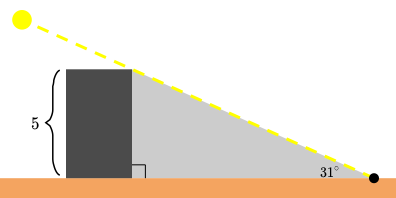
\includegraphics[width=0.5\textwidth]{../images/arquimedes.png}
    \end{center}
    \caption{Diagrama de la posición de Arquímedes (representado con un punto negro) con respecto a la gran roca.}
    \label{fig:arquimedes}
\end{figure}
Arquímedes sabía que a las 7 a.m. la luz del sol toca el suelo a un ángulo de 31$^\circ$.
La roca junto a la cual durmió mide 5 metros de altura.\\
\textbf{¿Qué tan lejos de la roca durmió Arquímedes?}\\
\textit{Redondea tu respuesta final a la centésima más cercana.}